\section{Machine Learning}

\begin{itemize}
\item What is machine learning?

\item Why is it useful for HEP? (Problems are multivariate... -- with high-order
  interactions between variables)

\item Supervised learning, i.e.\ have labelled data.

\item Binary classification tasks: Every training example has a label indicating
  the class membership. -> Focus on classification tasks

\item In HEP, the positive class is typically referred to as \emph{signal} while
  the negative class is referred to as \emph{background}.

\item What is training data, etc.

\item What is training.

\item Overfitting?
\end{itemize}


\subsection{Boosted Decision Trees}

Boosted decision trees (BDT) are classification and regression algorithms
composed of multiple \emph{decision trees}. This ensemble of decision trees is
created using an algorithm referred to as \emph{boosting}, which iteratively
fits shallow decision trees--or in general, any \emph{weak learning
  algorithm}--to altered versions of the training data. The training data is
modified at every iteration to emphasise errors made in previous
iterations. Finally, the predictions of the ensemble of trees are combined with
the goal of providing superior classification/regression performance compared to
a single decision tree. In the following a description of one of the BDT
algorithms implemented in \textsc{TMVA}~\cite{TMVA} is given, which is later
used in the search for Higgs boson pair production.


\subsubsection{Classification and Regression Trees}

Classification and regression trees~\cite{Breiman:1984jka,hastie09}, hereafter
collectively referred to as \emph{decision trees}, are used as the basis for
BDT. A decision tree partitions an $n$-dimensional space with coordinates
$\myvec{x} = (x_1, \dots, x_n)$ by recursively performing binary splits along
the coordinate axes until a stopping criterion is met. The resulting binary tree
structure and partitioning is illustrated in \Cref{fig:decision_tree} for a
two-dimensional example. A decision tree with $J$~leaf nodes partitions the
input space into $J$~mutually disjoint subregions denoted by $R_j$ for
$j = 1, \dots, J$. A constant value $c_j$ is assigned to every region $R_j$ such
that the prediction of a decision tree for a point~$\myvec{x}$ can expressed as
\begin{align*}
  h\bigl( \myvec{x}; \{c_j, R_j\}_{j=1}^{J} \bigr) = \sum_{j = 1}^{J} c_j \, \mathbf{1}(\myvec{x} \in R_j) \qquad \text{with} \qquad \mathbf{1}(\myvec{x} \in R_j) =
  \begin{cases}
    1, & \myvec{x} \in R_j \\
    0, & \text{else}
  \end{cases} \,\text{,}
\end{align*}
where $\{c_j, R_j\}_{j=1}^{J}$ fully specifies the decision
tree~\cite{hastie09}.

\begin{figure}[htbp]
  \centering

  \begin{subfigure}[b]{0.46\textwidth}
    \centering
    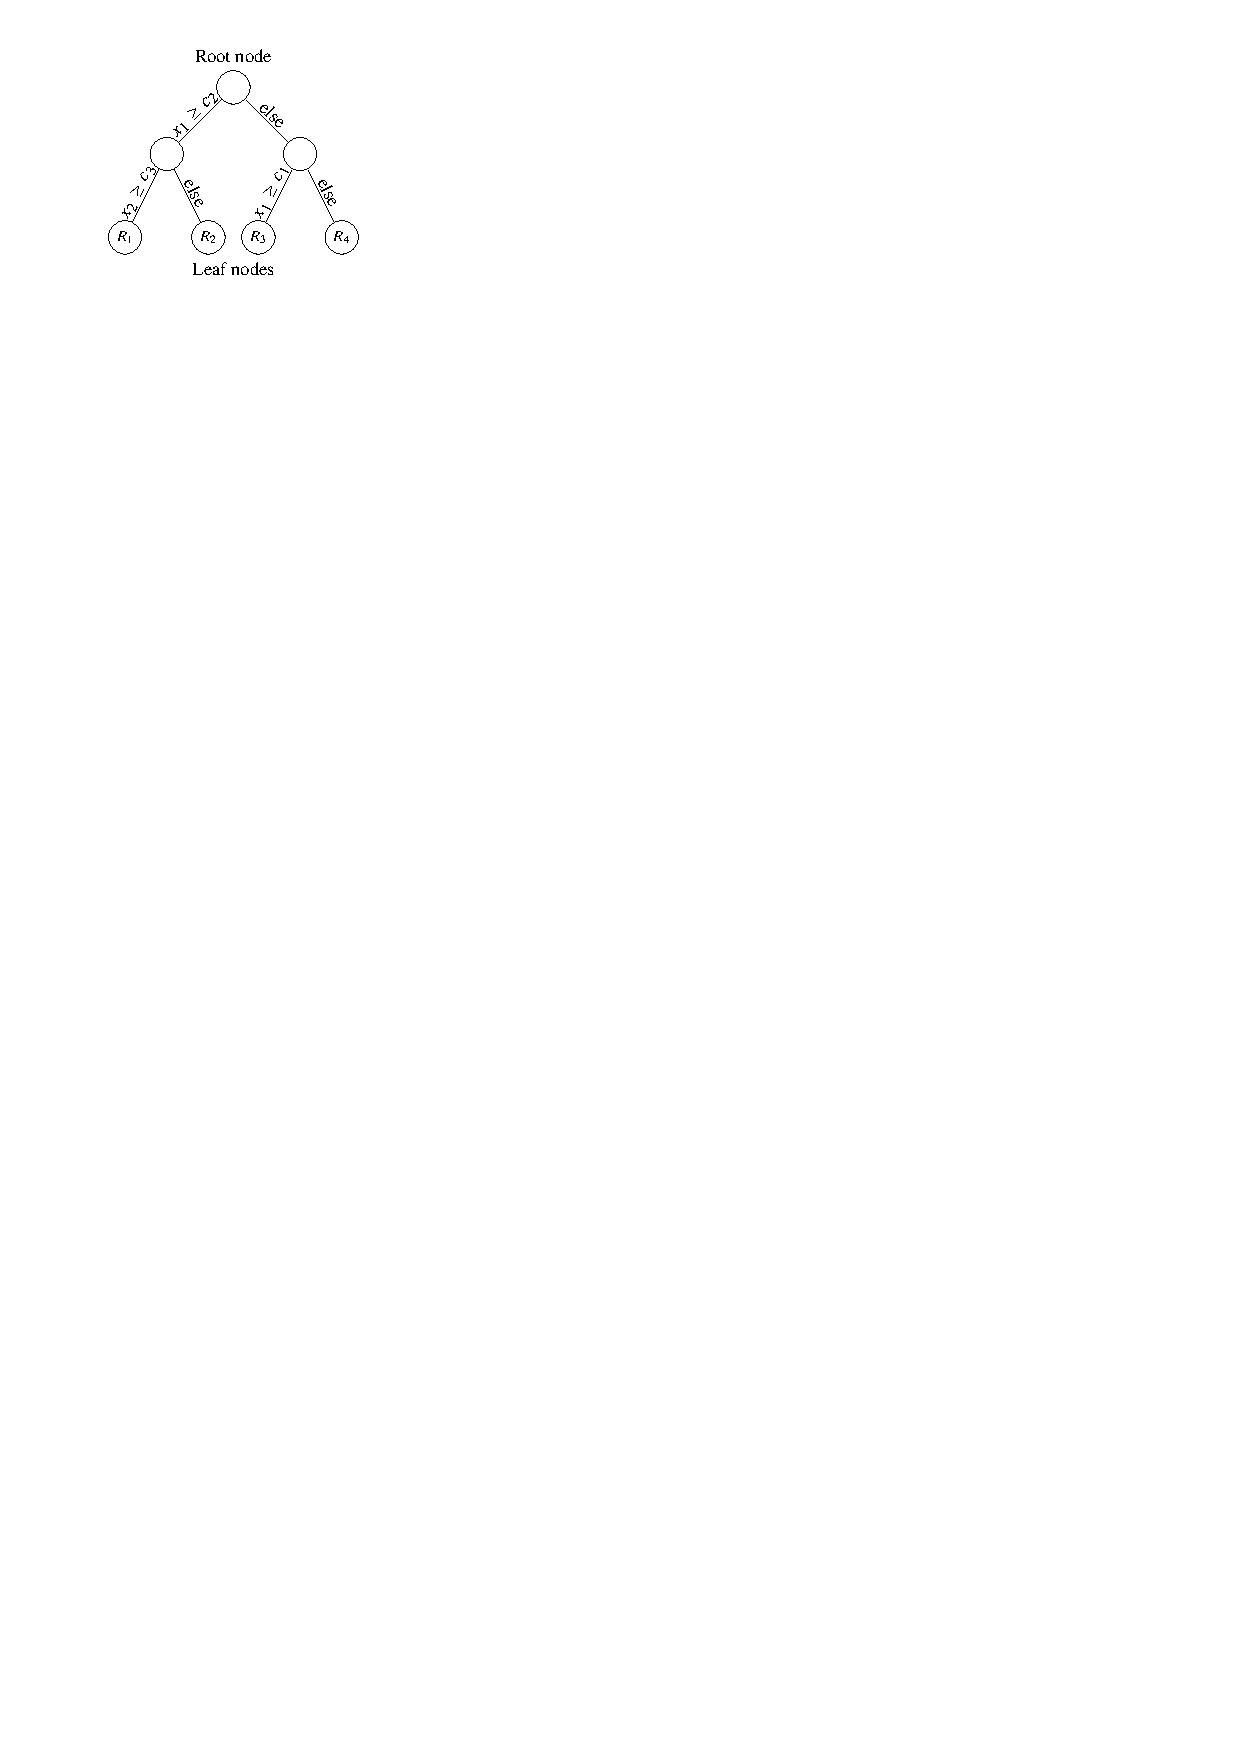
\includegraphics[scale=1.05]{ml/decision_tree}
    \caption{Binary tree structure of a decision tree.}
  \end{subfigure}\hfill%
  \begin{subfigure}[b]{0.46\textwidth}
    \centering
    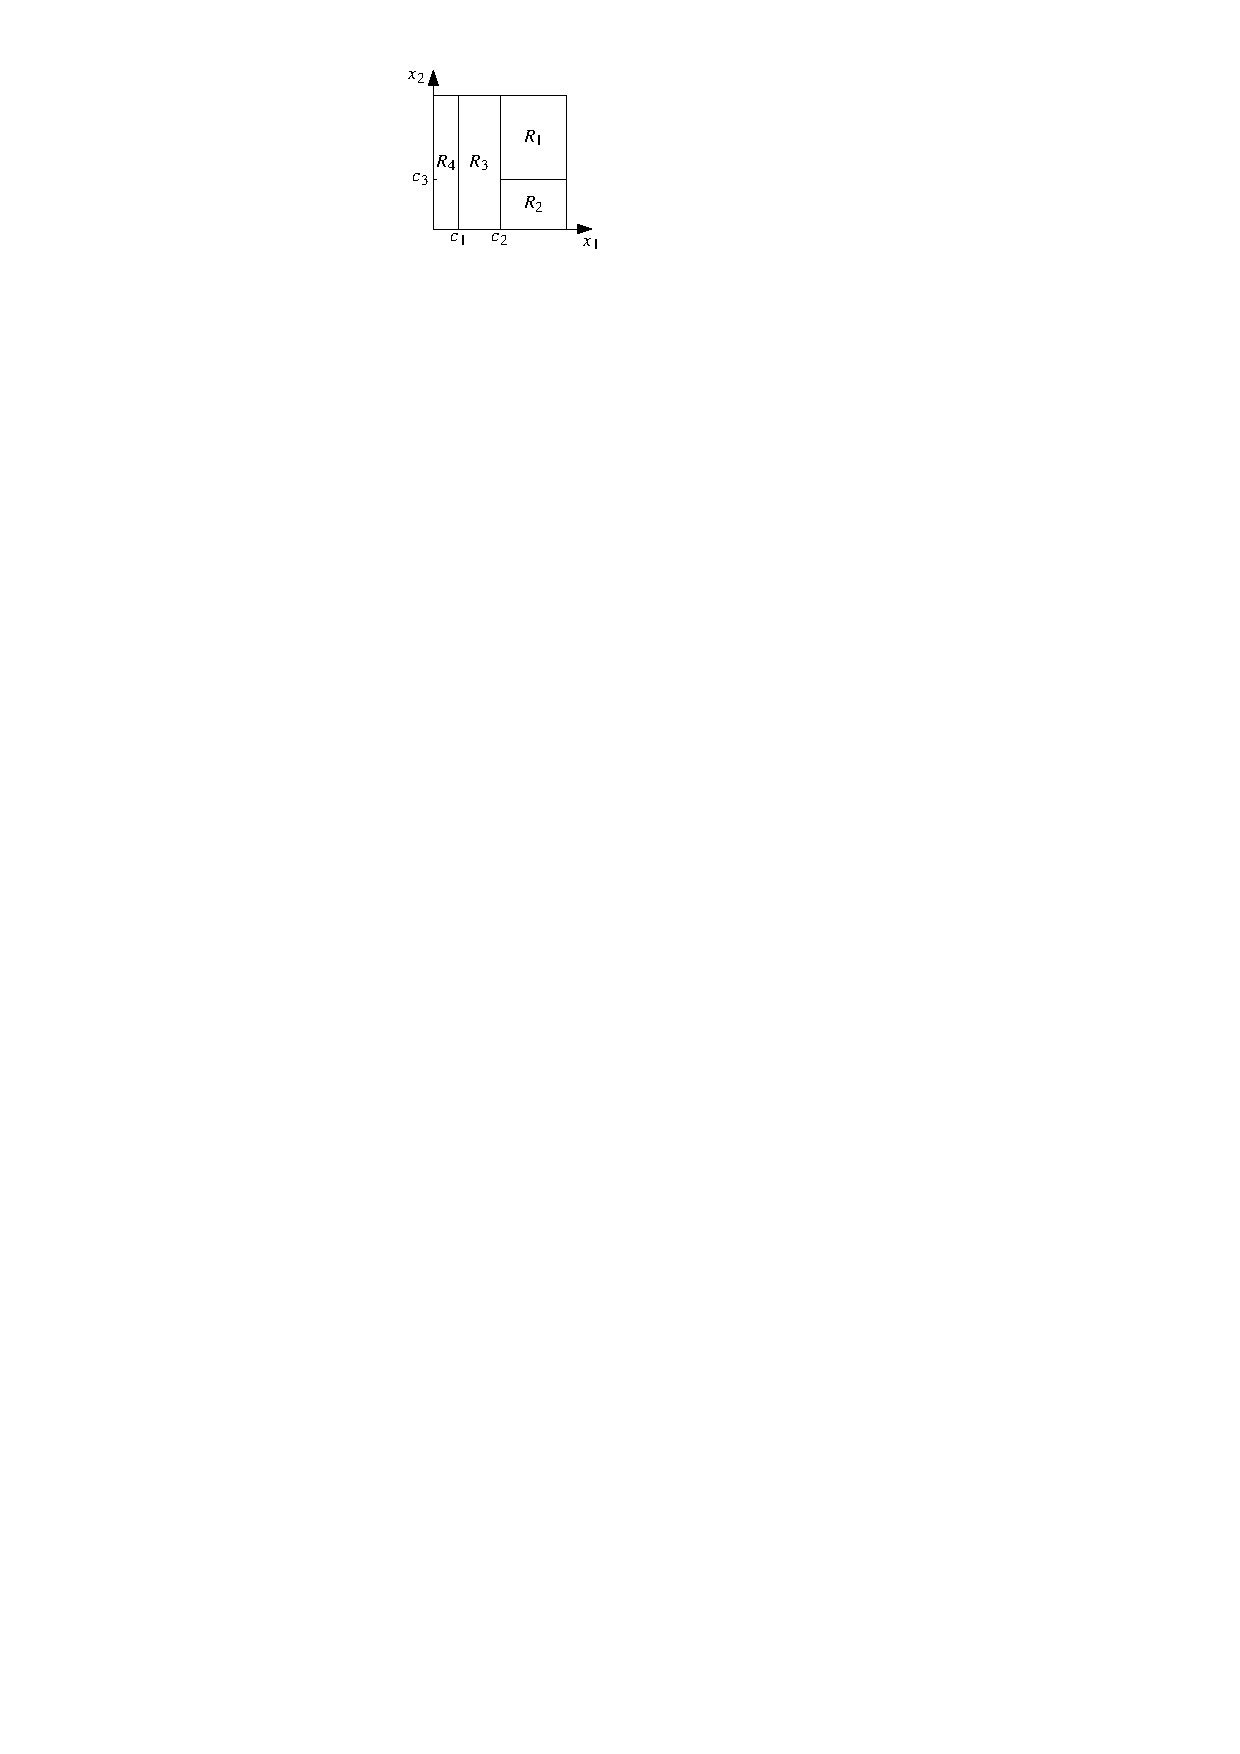
\includegraphics[scale=1.05]{ml/decision_tree_partitioning}
    \vspace*{0.7em}
    \caption{Partitioning resulting from the binary tree in (a).}
  \end{subfigure}\hfill%

  \caption{Example of a decision tree operating on a two-dimensional space with
    coordinates $\myvec{x} = (x_1, x_2)$. The tree has a depth of two and four
    leaf nodes that define the regions $R_1, \dots, R_4$. The figure is adapted
    from Ref.~\cite{hastie09}.}%
  \label{fig:decision_tree}
\end{figure}

Classification trees are constructed with the goal that the partitioning of the
input space yields subregions with low impurity, that is, the regions are mostly
populated by training examples of a single class. In this case, the impurity of
a tree node is quantified by the Gini index
\begin{align*}
  I_{\text{G}}(p) = 2 p (1 - p) \,\text{,}
\end{align*}
where $p$ is the proportion of examples from the positive class in a given
node~\cite{hastie09}. A \emph{greedy} strategy is adopted to grow decision trees
by performing the best possible split at every node. This split is determined by
minimising the weighted sum of Gini impurities of the resulting daughter nodes,
where impurities are weighted according to the total weight of training examples
populating a given node. In the classification case, the constants $c_j$
assigned to leaf nodes of the tree are either--depending on the algorithm
configuration--the proportion of examples from the positive class or the class
label of the majority class in a given leaf node.

Regression trees are constructed using a similar approach, however, with an
altered splitting criterion and different assignment of constants to leaf
nodes. Consider the split of a parent node into a left (L) and right (R)
daughter node. Let $(y, w)$ denote the tuple of regression target and weight of
a given training example. Moreover, let $T_{\text{L}}$ and $T_{\text{R}}$ denote
the set of $(y, w)$ for training examples populating the left and right daughter
node, respectively. The constants $c_{\text{L}}$ and $c_{\text{R}}$ assigned to
the daughter nodes are given by
\begin{align*}
  c_{\text{L}} = \frac{\sum_{(y, w) \in T_{\text{L}}} w y}{\sum_{(y, w) \in T_{\text{L}}} w} \qquad \text{and} \qquad c_{\text{R}} = \frac{\sum_{(y, w) \in T_{\text{R}}} w y}{\sum_{(y, w) \in T_{\text{R}}} w} \,\text{,}
\end{align*}
which is the weighted mean of the regression target for the training examples
populating the left and right node, respectively. The best possible split of a
node in a regression tree is chosen such that the squared error defined as
\begin{align*}
  \sum_{(y, w) \in T_{\text{L}}} w (y - c_{\text{L}})^2 + \sum_{(y, w) \in T_{\text{R}} } w (y - c_{\text{R}})^2
\end{align*}
is minimised.


\subsubsection{Boosting of Decision Trees}

Boosting is an approach of solving predictions tasks by constructing additive
models of the form
\begin{align*}
  F_{M}\bigl(\myvec{x}; \{ \beta_m, \gamma_{m} \}_{m=1}^{M} \bigr) = \sum_{m = 1}^{M} \beta_m b(\myvec{x}; \gamma_{m}) \,\text{,}
\end{align*}
where $\beta_m$ are coefficients and $b(\myvec{x}; \gamma_{m})$ are basis
functions parameterised
by~$\gamma_{m}$~\cite{Friedman:2000,Friedman:2001wbq}. While there is some
flexibility in choosing the family of basis functions, boosting is typically
applied to decision trees.
% Given a sample of training data, the model is fit using an
% iterative procedure in which the $m$-th stage of the model, which is given by
% \begin{align*}
%   F_{m}\bigl(\myvec{x}; \{ \beta_{n}, \gamma_{n} \}_{n=1}^{m} \bigr) = F_{m - 1}\bigl( \myvec{x}; \{ \beta_{n}, \gamma_{n} \}_{n=1}^{m-1} \bigr) + \beta_m b(\myvec{x}; \gamma_{m}) \,\text{,}
% \end{align*}
% is determined by choosing $\beta_{m}$ and $\gamma_{m}$ such that an objective
% function is improved~\cite{hastie09}. Notably, the $m$-th stage does not alter
% the parameters~$\{ \beta_{n}, \gamma_{n} \}_{n=1}^{m-1}$.
The following is concerned with a boosting algorithm referred to as
\emph{gradient boosting}~\cite{Friedman:2001wbq}. Gradient boosting is an
algorithm for constructing additive models that minimise arbitrary
differentiable loss functions, thus making it a useful tool for solving various
prediction tasks.

Consider a binary classification problem with predictors~$\myvec{X}$ and class
labels~$Y$, which are $Y = +1$ for the positive and $Y = -1$ for the negative
class. Both $\myvec{X}$ and $Y$ are random variables. Further, let
\begin{align}
  L(Y, F(\myvec{X})) = \ln\mathopen{}\left(
  1 + e^{-Y F(\myvec{X})}
  \right)\mathclose{}
  \label{eq:loss_gradboost}
\end{align}
be a loss function and $F$~a function of the predictors. The function that
minimises the expected loss is given by
\begin{align*}
  F^{*\!}(\myvec{x})
  = \argmin_F \, \expect[ L(Y, F) \mid \myvec{X} = \myvec{x} ]
  = \ln\mathopen{}\left(
  \frac{
  \mathbb{P}(Y = +1 \mid \myvec{X} = \myvec{x})
  }{
  \mathbb{P}(Y = -1 \mid \myvec{X} = \myvec{x})
  }
  \right)\mathclose{} \,\text{,}
  %\label{eq:gradboost_logodds}
\end{align*}
which are the conditional log-odds of an observation with predictors~$\myvec{x}$
belonging to the positive class~\cite{Friedman:2000}. Knowledge of $F^{*\!}$
would solve the classification task since
\begin{align}
  \mathbb{P}(Y = +1 \mid \myvec{X} = \myvec{x}) = \frac{1}{1 + e^{-F^{*\!}(\myvec{x})}}
  \qquad \text{and} \qquad
  \mathbb{P}(Y = -1 \mid \myvec{X} = \myvec{x}) = \frac{1}{1 + e^{+F^{*\!}(\myvec{x})}} \,\text{,}
  \label{eq:gradboost_probas}
\end{align}
thus motivating the choice of loss function in \Cref{eq:loss_gradboost} for
binary classification.

% Gradient boosting can be used to find an additive model that minimises this
% loss function for a finite sample,

% with this loss function can be used to
% find an approximation to $F^{*\!}(\myvec{x})$

% with decision trees can be used to find an approximation to
% $F^{*\!}(\myvec{x})$ using a finite sample of training data.

An algorithm referred to as \textsc{TreeBoost} proposed by
Friedman~\cite{Friedman:2001wbq} is outlined. \textsc{TreeBoost} uses gradient
boosted decision trees and the loss function in \Cref{eq:loss_gradboost} to fit
a binary classifier to a sample of training data. A version of this algorithm is
employed in \textsc{TMVA}~\cite{TMVA}, which provides the BDT implementation
used in this thesis. The description is based on Ref.~\cite{Friedman:2001wbq}
with some modifications (e.g.\ allowing training data to be weighted).

\vspace{11pt}
\noindent\textbf{\textsc{TreeBoost} algorithm for binary classification} \\[11pt]
\noindent Inputs:
\begin{itemize}[itemsep=2pt]
\item Training data $\{(\myvec{x}_i, y_i, w_i)\}_{i = 1}^{N}$ with
  predictors~$\myvec{x}_i$, class labels $y_i$, and weights~$w_i$.
\item Number of boosting iterations $M$.
\item Shrinkage parameter~$\eta$ ($0 < \eta \leq 1$).
\item Hyperparameters of the regression tree algorithm.
\end{itemize}

\vspace{6pt}
\noindent Algorithm:
\begin{enumerate}[itemsep=2pt]

\item The model is initialised to make a constant prediction according to
  \begin{align*}
    F_0(\myvec{x}) = \ln\mathopen{}\left( \frac{1 + \bar{y}}{1 - \bar{y}}
    \right)\mathclose{}
    \qquad \text{with} \qquad
    \bar{y} = \frac{\sum_{i=1}^{N} w_i y_i}{\sum_{i=1}^{N} w_i} \,\text{,}
  \end{align*}
  which are the (unconditional) log-odds of $Y = +1$ estimated using the
  training data.

\item For $m = 1$ to $M$:
  \begin{enumerate}[itemsep=2pt]

  \item Calculate the pseudo-residuals
    \begin{align*}
      r_i
      = - \left. \frac{\partial L(y_i, F(\myvec{x}_i))}
      {\partial F(\myvec{x}_i)}\right|_{F(\myvec{x}_i) = F_{m - 1}(\myvec{x}_i)}
      \overset{\text{Eq.\ (\ref{eq:loss_gradboost})}}{=}
      %\frac{y_i}{1 + \exp(y_i F_{m-1}(\myvec{x}_i))}
      \frac{y_i}{1 + e^{y_i F_{m-1}(\myvec{x}_i)}}
    \end{align*}
    for all training examples.
    % , where $\myvec{x}_i$ are the predictors and $y_i$ the class label of the
    % $i$-th training example, respectively.

  \item Fit a regression tree to the training data to estimate the
    pseudo-residuals using the predictors~$\myvec{x}$. The prediction of the
    fitted regression tree is denoted by
    $h\bigl( \myvec{x}; \{c_{jm}, R_{jm}\}_{j=1}^{J_{m}} \bigr)$, where $J_{m}$
    is the number of leaf nodes, $c_{jm}$ is the constant predicted by the
    $j$-th leaf node, and $R_{jm}$ is the region defined by the $j$-th leaf
    node.

  \item The leaf node constants of the regression tree,
    $\{c_{jm}\}_{j=1}^{J_{m}}$, are updated to minimise
    \begin{align*}
      \sum_{i=1}^{N} w_i \cdot
      L\mathopen{}\left( y_i, F_{m - 1}(\myvec{x}_i)
      + h\bigl( \myvec{x}_i; \{c_{jm}, R_{jm}\}_{j=1}^{J_{m}} \bigr)
      \right)\mathclose{}
      \,\text{,}
    \end{align*}
    where the sum goes over all training data. This optimisation problem has no
    analytical minimiser for the loss function in
    \Cref{eq:loss_gradboost}. Instead, the $\{c_{jm}\}_{j=1}^{J_{m}}$ are chosen
    to approximately minimise the above criterion by performing a single step of
    Newton's method.\footnote{The starting point for Newton's method is taken to
      be $c_{jm} = 0$ for all leaf nodes.} This yields the updated leaf node
    constants
    \begin{align*}
      c_{jm}^\prime = \frac{ \sum_i w_i r_i }{ \sum_i w_i |r_i| (1 - |r_i|)} \,\text{,}
    \end{align*}
    where the sum goes over the training data populating the $j$-th leaf node of
    the tree. This step is specific to the \textsc{TreeBoost} algorithm by
    Friedman.

  \item Determine the $m$-th stage of the model by setting
    \begin{align*}
      F_m(\myvec{x}) = F_{m - 1}(\myvec{x})
      + \eta \cdot h\bigl( \myvec{x}; \{c_{jm}^\prime, R_{jm}\}_{j=1}^{J_{m}} \bigr)
      \,\text{,}
    \end{align*}
    where $\eta$ is a parameter of the boosting algorithm referred to as the
    \emph{shrinkage} or \emph{learning rate}. Generally, the shrinkage is set to
    values below unity such that every stage of boosting performs a suboptimal
    update. This serves as a form of regularisation to prevent overfitting.

  \end{enumerate}

\item The final prediction of the boosting procedure,
  $F_{M\hspace{-0.07em}}(x)$, can be used to estimate the probability
  $\mathbb{P}(Y = +1 \mid \myvec{X} = \myvec{x})$ according to
  \Cref{eq:gradboost_probas} as
  \begin{align*}
    p(\myvec{x}) = \frac{1}{1 + e^{-F_{M\hspace{-0.07em}}(\myvec{x})}} \,\text{.}
  \end{align*}
  In HEP, this quantity is commonly referred to as the \emph{BDT score}.

\end{enumerate}
This algorithm is reminiscent of the classical gradient descent algorithm for
minimisation, however, in the case of gradient boosting the optimisation is
performed in the space of functions instead~\cite{Friedman:2001wbq}. Steps 2a)
and 2b) of the algorithm serve to estimate the negative gradient of the loss
function with respect to $F(\myvec{x})$, which is evaluated at the function
estimate of the previous boosting iteration. In gradient descent, the step size
of the update is often determined by performing a line search along the
direction of steepest descent. This is the task of step 2c) in which the step
size is determined, however, for \textsc{TreeBoost} the size of the gradient
descent step is determined on a per-leaf basis. Finally, step 2d) performs the
(regularised) gradient descent update.


\subsection{Neural Networks}%
\label{sec:neural_networks}

Neural networks (NNs) can be interpreted as functions defined by the composition
of multiple, usually non-linear, parametric functions. They can represent a rich
class of functions, motivating their use as function
approximators~\cite{hornik1989multilayer}. An illustrative example of an NN is
the \emph{multilayer perceptron} (MLP). The basic element of MLPs--and many
other types of NNs--are \emph{densely connected layers} that apply
transformations of the form
\begin{align}
  f_i(\myvec{x}; \myvec{W}_i, \myvec{b}_i) = \phi_i(\myvec{W}_i \myvec{x} + \myvec{b}_i) \,\text{,}
  \label{eq:dense_layer}
\end{align}
where $\myvec{x}$ is the layer input, $\myvec{W}_i$ and $\myvec{b}_i$ are the
weights and biases, respectively, and $\phi_i$ is an activation function that is
applied element-wise. An MLP with $N$~hidden layers is given by the composition
of $N + 1$ functions of the form displayed in \Cref{eq:dense_layer}, such that
the output of the MLP can be expressed as
\begin{align*}
  f\bigl( \myvec{x}; \{\myvec{W}_{i},\myvec{b}_{i} \}_{i=1}^{N+1} \bigr)
  = \bigl( f_{N+1} \circ \dots \circ f_{1} \bigr)
  \bigl( \myvec{x}; \{\myvec{W}_i, \myvec{b}_i\}_{i=1}^{N+1} \bigr)
  \,\text{.}
\end{align*}
In general, the structure of NNs can be more complex than illustrated in this
example. Therefore, the \emph{architecture} of a NN is frequently expressed as a
directed graph with nodes representing functions/layers and edges defining how
functions/layers are composed.

% For the MLP example, this graph is
% \begin{align*}
%   (\myvec{x} \to) \, \text{Dense}_{1} \to \dots \to \text{Dense}_{N + 1}
% \end{align*}
% where $\text{Dense}_{i}$ denotes the $i$-th densely connected layer, and
% $\myvec{x}$ represents the input to the MLP. The $(N+1)$-th densely connected
% layer is also referred to as the output layer.

The ability of NNs to approximate a large class of functions makes them
attractive candidates for machine learning applications. Hereafter, the
prediction of a generic NN is denoted by $f(\myvec{x}; \myvec{\theta})$, where
$\myvec{x}$ is the NN input and $\myvec{\theta}$ are its parameters. Consider a
binary classification problem with predictors~$\myvec{X}$ and class labels~$Y$,
which take the values of $Y = 1$ and $Y = 0$ for the positive and negative
class, respectively. A suitable loss function for binary classification is
\begin{align}
  L(Y, f(\myvec{X}; \myvec{\theta})) =
  \begin{cases}
    -\ln\mathopen{}\left( f(\myvec{X}; \myvec{\theta}) \right)\mathclose{},       & Y = 1 \\
    -\ln\mathopen{}\left( 1 - f(\myvec{X}; \myvec{\theta}) \right)\mathclose{},   & Y = 0 \\
  \end{cases} \,\text{,}
  \label{eq:loss_bce}
\end{align}
where it is assumed that the NN can be defined such that
$f(\myvec{x}, \myvec{\theta}) \in (0, 1)$, for example by using the logistic
(sigmoid) function as the activation function in the final layer. This loss
function is referred to as the \emph{binary cross-entropy loss}, hereafter. The
function that minimises the expected loss is
\begin{align*}
  f^{*\!}(\myvec{x})
  = \argmin_{f} \expect[ L(Y, f) \mid \myvec{X} = \myvec{x} ]
  = \mathbb{P}(Y = 1 \mid \myvec{X} = \myvec{x}) \,\text{,}
\end{align*}
motivating the use of \Cref{eq:loss_bce} as a loss function for binary
classification.\footnote{The loss function in \Cref{eq:loss_bce} is similar to
  the one used for binary classification with gradient boosted trees in
  \Cref{eq:loss_gradboost}. This is due to both being derived from the negative
  log-likelihood of the Bernoulli distribution (the distribution of $Y$). The
  only differences are the change in class labels ($Y \in \{-1, 1\}$ for boosted
  trees, $Y \in \{0, 1\}$ for NNs) and the fact that the ensemble of trees
  approximates the conditional log-odds of $Y = 1$ while the NN estimates the
  conditional probability of $Y = 1$, directly.}

The binary classification task can be solved by approximating
$f^{*\!}(\myvec{x})$ using an NN with parameters set such that the mean loss
over a sample of training data~$\{\myvec{x}_i, y_i, w_i\}_{i = 1}^N$ is
minimised. Formally, the parameters are given by the optimisation problem
\begin{align*}
  \myvec{\hat{\theta}} =
  \argmin_{\myvec{\theta}}\mathopen{}\left(
  \frac{\sum_{i = 1}^{N} w_i L(y_i, f(\myvec{x}_i; \myvec{\theta}))}{\sum_{i = 1}^{N} w_i}
  \right)\mathclose{}
  \,\text{.}
\end{align*}
This optimisation is non-convex and analytically intractable (for non-trivial
NNs). In practice, the minimisation is often performed using \emph{stochastic
  gradient descent} (SGD) or derivatives thereof. SGD is a gradient-based
optimisation method in which the gradient of the loss function is estimated
using random subsamples of training data. These subsamples are referred to as
\emph{mini-batches} and are denoted by
$\{\myvec{x}_{(i)}, y_{(i)}, w_{(i)}\}_{i=1}^{M}$ for a batch of size
$M$~\cite{Goodfellow-et-al-2016}. The mini-batch estimate of the gradient is
given by
\begin{align*}
  \myvec{g}(\myvec{\theta})
  = \frac{
  \sum_{i=1}^{M} w_{(i)}  \nabla_{\!\myvec{\theta}} L(y_{(i)}, f(\myvec{x}_{(i)}; \myvec{\theta}))
  }{
  \sum_{i=1}^{M} w_{(i)}
  } \,\text{,}
\end{align*}
where $\nabla_{\!\myvec{\theta}}$ refers to the vector of partial derivatives in
parameter space~\cite{Goodfellow-et-al-2016}. The training of NNs using SGD
proceeds by first randomly initialising the parameters to
$\myvec{\theta} = \myvec{\theta}_0$. Afterwards, a number of SGD iterations are
performed until convergence or another stopping criterion is met. The iterations
consist of drawing a mini-batch from the training data followed by the parameter
update
\begin{align*}
  \myvec{\theta}_{t + 1} = \myvec{\theta}_{t} - \eta_{t} \myvec{g}(\myvec{\theta}_{t}) \,\text{,}
\end{align*}
where $\eta_{t}$ is referred to as the learning
rate~\cite{Goodfellow-et-al-2016}. The learning rate can follow a predefined
schedule with respect to the iteration counter~$t$, common ones being constant
or exponentially decaying learning rates. A modification of this algorithm is
\emph{SGD with momentum} which aims to improve the convergence properties of
SGD. The modified algorithm alters the parameter update according to
\begin{align*}
  \myvec{\theta}_{t + 1} = \myvec{\theta}_{t}
  + \alpha \Delta\myvec{\theta}_{t} - \eta_t \myvec{g}(\myvec{\theta}_{t})
  \qquad \text{with} \qquad
  \Delta\myvec{\theta}_{t} =
  \begin{cases}
    \myvec{\theta}_{t} - \myvec{\theta}_{t - 1}, & t > 0 \\
    0,                                         & t = 0
  \end{cases}
\end{align*}
which introduces the momentum parameter
$0 \leq \alpha < 1$~\cite{rumelhart1986learning,Goodfellow-et-al-2016}. The
update of SGD with momentum can be loosely interpreted as the movement of a
massive object through parameter space with two forces acting on the object: a
force proportional to~$-\myvec{g}(\myvec{\theta})$ and a friction-like force
proportional and opposed to the
velocity~$\Delta\myvec{\theta}_{t}$~\cite{Goodfellow-et-al-2016}.


\subsubsection{Recurrent Neural Networks}%
\label{sec:rnn}

Another appealing feature of NNs is the ability to process various forms of
structured data--e.g.~graphical images or natural language--by employing
specialised network architectures. Among these architectures are \emph{recurrent
  neural networks} (RNN), which allow to operate on ordered, variable-length
sequences. Such sequences occur in many scenarios, an example from natural
language processing being the representation of sentences, which are sequences
of words. In the context of HEP, one might encode the properties of jets
reconstructed in an particle collision event as a variable-length sequence.



Internal state -> contextual information

Formally, variable-length sequences will be denoted by

$\myvec{x} = (\myvec{x}_{t})_{t = 1}^{N}$

in the following, where the length of the sequence~$N$ is allowed to vary
between data points.



Long short-term memory (LSTM)~\cite{lstm}


\cite{lstm,Goodfellow-et-al-2016,keras}


three gates: the forget gate, the input gate, and the output gate.


\begin{alignat*}{3}
  \myvec{f}_{t}(\myvec{x}_{t}, \myvec{h}_{t-1}) &= \myvec{\sigma}(\myvec{U}_{\text{f}} \kern1pt \myvec{x}_{t} &&+ \myvec{W}_{\text{f}} \kern1pt \myvec{h}_{t - 1} &&+ \myvec{b}_{\text{f}}) \\
  \myvec{i}_{t}(\myvec{x}_{t}, \myvec{h}_{t-1}) &= \myvec{\sigma}(\myvec{U}_{\text{i}} \kern1pt \myvec{x}_{t} &&+ \myvec{W}_{\text{i}} \kern1pt \myvec{h}_{t - 1} &&+ \myvec{b}_{\text{i}}) \\
  \myvec{o}_{t}(\myvec{x}_{t}, \myvec{h}_{t-1}) &= \myvec{\sigma}(\myvec{U}_{\text{o}} \kern1pt \myvec{x}_{t} &&+ \myvec{W}_{\text{o}} \kern1pt \myvec{h}_{t - 1} &&+ \myvec{b}_{\text{o}})
\end{alignat*}

The activations of the gates control the flow of information

\begin{align*}
  &\myvec{c}_{t} = \myvec{f}_{t} \circ \myvec{c}_{t - 1}
    + \myvec{i}_{t} \circ \myvec{\phi}(\myvec{U} \myvec{x}_{t} + \myvec{W} \myvec{h}_{t-1} + \myvec{b}) \\
  &\myvec{h}_{t} = \myvec{o}_{t} \circ \myvec{\phi}(\myvec{c}_{t})
\end{align*}

\begin{figure}[htbp]
  \centering

  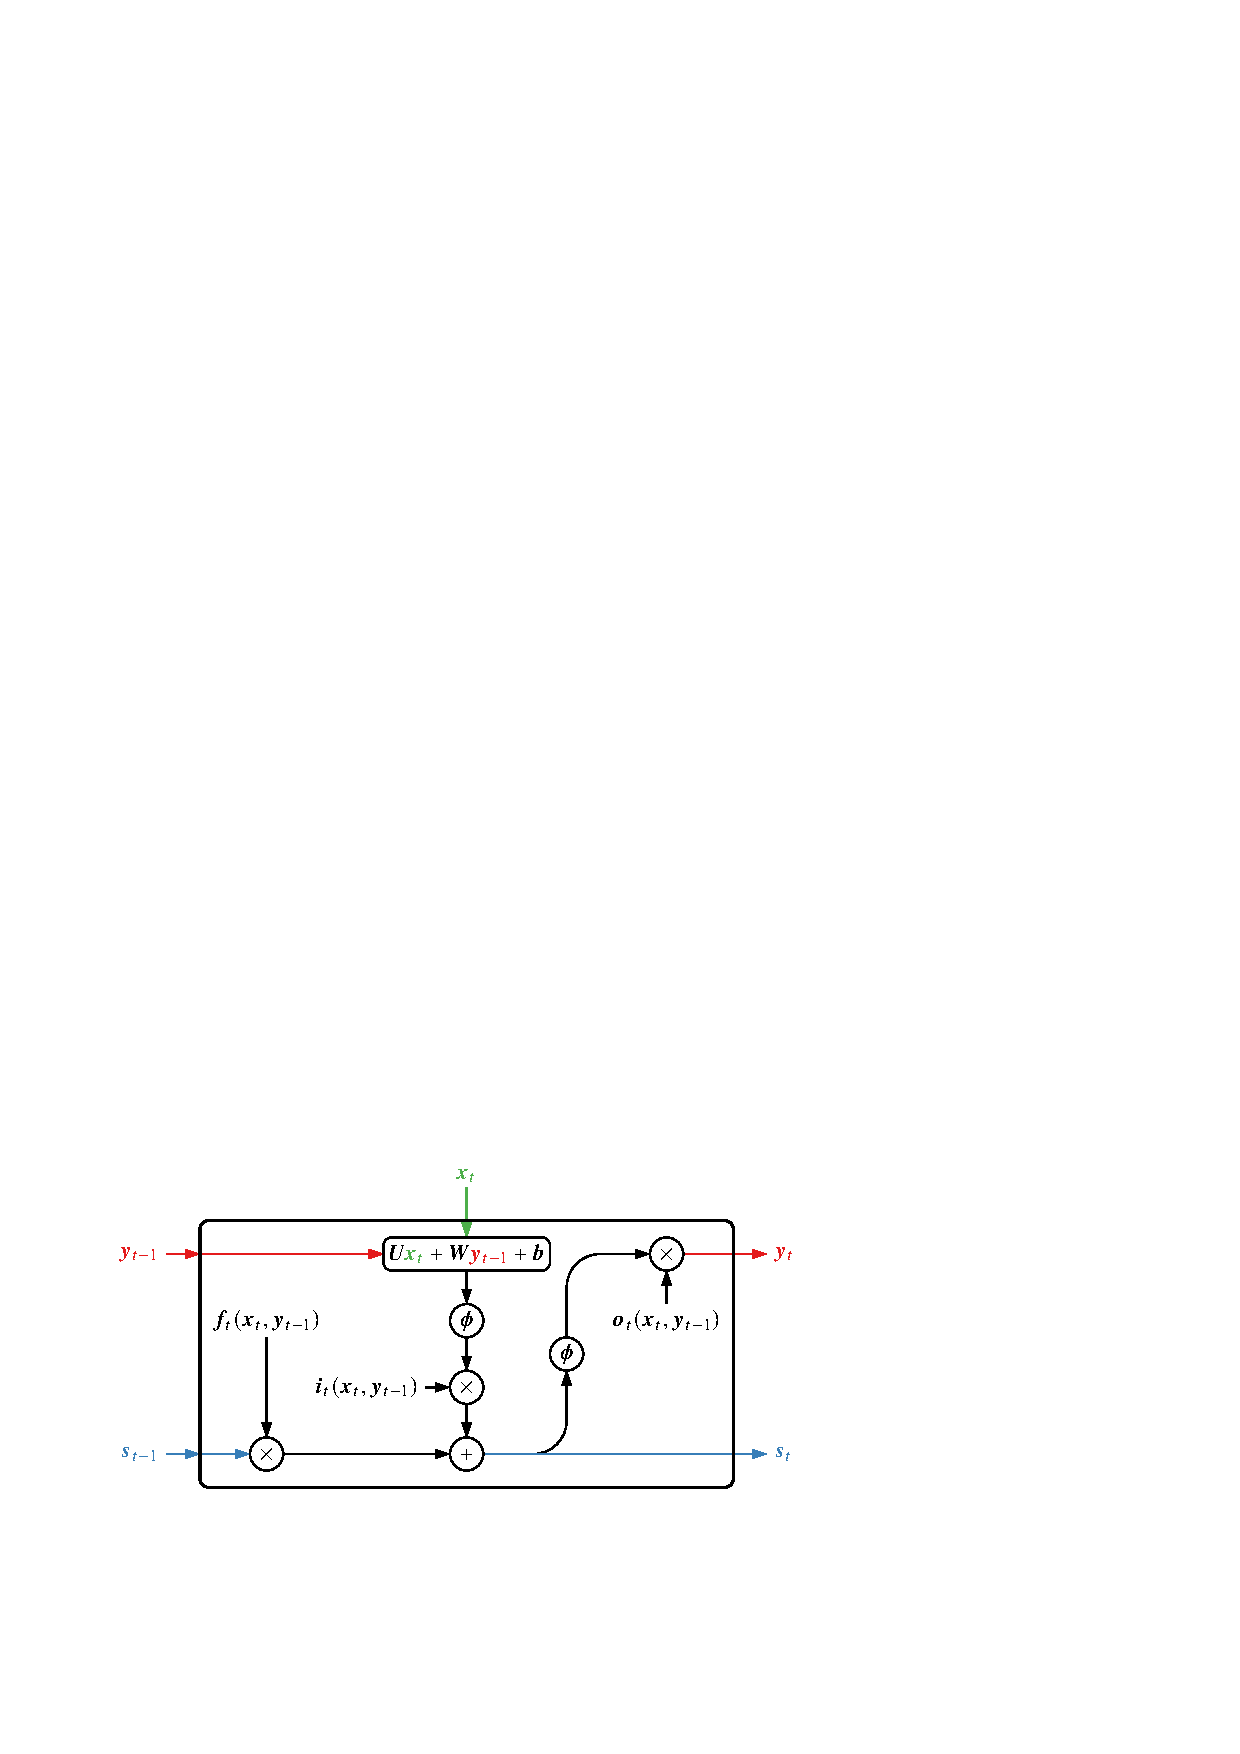
\includegraphics[scale=1.0]{ml/lstm}

  \caption{Computational graph of a single LSTM cell for time step
    $t$. Operations in circles represent element-wise multiplication
    ($\times$), element-wise addition ($+$), and element-wise application of the
    $\tanh$ activation function ($\myvec{\phi}$).
  }
  \label{fig:lstm}
\end{figure}






% A input sequence~$(\myvec{x}_{t})_{t = 1}^{N}$ can be processed by connecting
    % repeating the computation depicted in the figure once for
    % connecting $N$ of the depicted cell as depicted horizontally
    % horizontally connecting $N$.




RNN operates on sequences of vectors. The length of the sequence is
variable. Each element of the sequence is typically referred to as a \emph{time
  step}.

Can be unfolded into a feedforward neural network. Main point: The unfolded
layers share their parameters (otherwise the sequences would have to have fixed
length).


Gated RNNs solve the vanishing or exploding gradient problems that plague naive
RNN implementations. Gradients exponentially decay or grow with every time step.


%%% Local Variables:
%%% mode: latex
%%% TeX-master: "../../phd_thesis"
%%% End:
